\documentclass[tikz,border=7mm]{standalone}
\usetikzlibrary{angles}
\begin{document}
  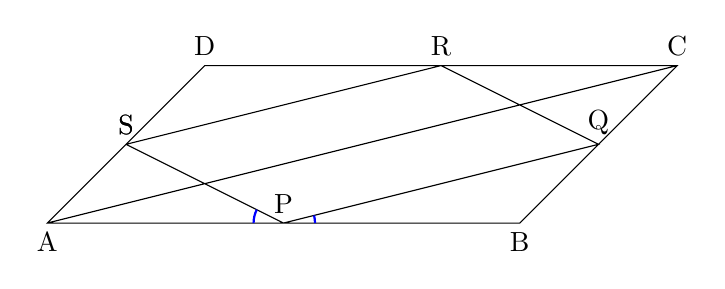
\begin{tikzpicture}[xslant=1,xscale=3,scale=2]
    \draw (0,0) rectangle
          (1,1) coordinate(C) node[above]{C} -- (0,0) coordinate(A) node[below]{A}
          (1,0) coordinate(B) node[below]{B}  
          (0,1) coordinate(D) node[above]{D}
          (0,0.5) coordinate(S) node[above]{S} --(0.5,0) coordinate(P) node[above]{P} --(1,0.5) coordinate(Q) node[above]{Q} --(0.5,1) coordinate(R) node[above]{R} --(0,0.5) coordinate(S) node[above]{S} 
          pic[draw,blue,thick,angle radius=4mm] {angle = B--P--Q}
          pic[draw,blue,thick,angle radius=3.8mm] {angle=S--P--A};
          pic[draw,black,thick,angle radius=3.8mm] {angle=B--Q--P};
  \end{tikzpicture}
\end{document}